%% ----------------------------------------------------------------
\chapter{Project Management}
%% ----------------------------------------------------------------
Project management goes here...

\section{Gantt Charts}
Michael
Place Gantt charts here.

\section{Risk Management}
Mitch
Place risk management considerations and compare with risks encountered.

\section{Work Allocation}

Working in a group has its advantages, but it also has drawbacks. The group has more man power and time, but the effectiveness of work allocation and other management skills must be achieved. Therefore, to use all the human resources as competent as possible. Although the developers have known about the specification of the project well, it is not so obvious how to implement the entirely approach to the project that is driven by some device which the members never have seen it before such as camera module, and the UAV. The following factor has been considered thoroughly before assigning task to any team members:

\begin{itemize}
\item	Availability of each member.

\item	The resource limitation
 
\item	The clarification of the task

\item   Time allowance for unexpected problems

\item	Each individual skills
\end{itemize}

\begin{figure}[!hbtp]
\begin{center}
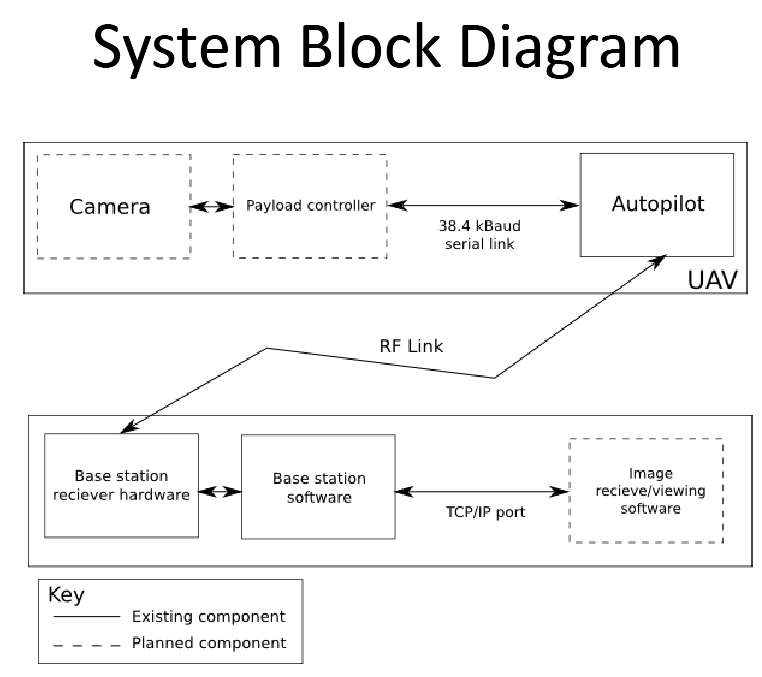
\includegraphics[scale=0.6]{SystemBlockDiagram.PNG} 
\caption{The system final diagram\label{systemBlocD}}
\end{center}
\end{figure}


\subsection{Planned Work Allocation}
 It is very essential that each member other coursework deadline and exams include in the consideration of work allocation. 
The engineer will work effectively if they got assigned  to their interest in the duty and that role clarified well. The work assign to each individual will be based on the posses sufficient skill and knowledge to perform the task. However, the team members must have flexibility in their time in order to support other team members when they have problems. Each task has been assigned a task leader and it will have the another member set to the same task in case the task leader has problems with the work they have done. In order to avoid work over run the time, the project has been set an earlier deadline so that if any unexpected problems happen, there are still a spare time to solve the problem. The specific skills that individuals want to mention are:

\begin{itemize}
\item Andy: Power, PCB, Control, MATLAB
\item Mitch: Image Processing, MATLAB, ASM, Report Writing
\item John: MATLAB, Image Processing, Control, Radio Transmission
\item Peak: Digital Control, Display, MATLAB, Information Theory
\item Michael: Programming, $\mu$Processors, Interfaces
\end{itemize}

Each member has variety of skills. Therefore the task has been located to each person according to this list.

The time line of the task is also important because some task for each individual depend on a completion of another task. This cause problems when one task got stuck and so the productiveness of the time management will be reduced. This can be solved by assigning another task that is not dependant on the other tasks. 

A Resource limitation is one of the factor that limited the group member to do tasks. This is because the customer provide only a single UAV and also only one camera has been purchased, so only one person can work on this device at a time. We solved this problem by having a laboratory space that the UAV will be placed their all the time so any of the team member can access it. To mange the limited resource, the only time that the individual access the UAV is when he wants to test the system. 

To clarify the tasks so the individuals can understand and also to ensure that all the tasks have been assigned is essential. The real development of this project will analyze the requirement from the start of how the project could be ensemble. The project will be a bottom-up design. It will start from each individual completion of a small task and then integrate them into a successful complete project. 



\subsection{Actual Task Allocation}

In the real work environment, the unexpected situation happens at all time. Each members of the group face different problem, some problem is easy to solved but some is very difficult and time consuming. The back up plan and unplanned problem solving skills is needed. Although many problems happens, but all the team members have been flexible to support each other and most main problems have been solved.

Figure\ref{systemBlocD} shows a block diagram of the whole system that the developers has slitted in to blocks of tasks. 
The camera module and other hardware have uncontrollable acquiring time. Some of the group members has problem with the delay of the hardware deliveries. Therefore, the time has to extended longer than the gantt chart. The solution to this is the software has been developed according to the camera sheet of the hardware. And at this stage, the background reading is very necessary so the developers has used this waiting time to plan and develop the software, so when the components arrive, all the task can be implemented.

The task that depend on acquiring the camera are the communication between the payload and the camera,prototype camera module, and image encoding. The problem that the developers have is the camera delivered is a faulty.These tasks has been suspended until the camera have arrived.  Therefore, the new camera has to be purchased and the allocation of work is necessary. There are part that is not depended on the hardware such as encoding/decoding images, and ground station software. So the members who were assigning to work on the camera has been allocate to do the software part first.

The payload controller has the problem with the hardware part of the UAV. The payload did not respond to the UAV signal at first. Therefore, we assign another group member to support this problems. The task leader of this has been assigned to do another software module which have to be implemented. This problem also need a support from the customer to update the UAV firmware. After the problem have been noticed, it has been solved successfully. 

The SD card memory task was considered as a small task in the planned work, but in the real implementation it is very important. Therefore, we assign on of the member responsible to this task. The SD started to implemented after the camera have been arrive and implemented correctly. 

Because there is only one camera purchased, only one member of the team assign to keep the camera. There are problems with the cameras including the delay of deliveries, and camera faulty. The task leader of this has been assign to research on the progressive image on MATLAB in order to make a prototype presentation of a compression image taken. The task has been delayed from the time set to an individual. But after the second working camera arrived, the task has been done beautifully and there is enough time to combine with other tasks.

\section{Team Resources}
John
What we used to get the job done...

\subsection{Budget}
What did we need to buy in the end?

\subsection{Electronic Material}
Did we make use of anything electronic that we had before the project?

\section{Group Communication}
Andy
Talk about how the group contacted each other (email, meetings, mobiles)...



\subsection{Formal Meetings}
Talk about the usefulness and benefit of the formal Tuesday meetings...

For the duration of the project, we held weekly meetings on most Tuesday 
Afternoons from 4pm onwards in the Hartley Library. This allowed us to 
review progress made against progress expected, and to modify our project 
plan and allocation of work for the following week.
\\
Minutes of these meetings are available both in our repository \cite{github} 
(documents/minutes), and as an appendix ?????
\\
The timing of these (the afternoon before our weekly meetings with our 
supervisor) was also quite useful, as it allowed us to present a clear outline 
of new developments and our plans week-by-week.

\subsection{Methods of Communication}
Talk about which methods were used more often, which were useful...

The group has used various methods of communication during the project: 
email, 

\subsection{Source Control}
How we used e-mails, SVN Tortoise, and Github to keep our progress safe...

We decided to use version control software throughout the project, to manage 
everything from minutes to source code and payload schematics. As well as 
being a very useful tool to facilitate group work, it also helps us to meet 
our customer's request to deliver this as an open source project - at the end 
of the project, a repository could easily be gardened and presented, with the 
addition of appropriate open-source licenses at the end of the project.
\\
Initially, we used a central Subversion (SVN) repository hosted on ECS' 
UGForge service. It was decided to use this as most of the group had 
experience using SVN. This worked well for most of the project, but 
unfortunately, something was committed to this repository that could not be 
open sourced (the customer's Ground Control Station software). This presented 
us with a problem, as although it would be trivial to revert this commit with 
the "\$ svn merge" command, this creates a new commit, and the file in 
question would remain in the repository's history and could still be accessed.
\\
In theory, it would be possible to remove this commit from SVN history by 
using the "\$ svnadmin dump" command, filtering the offending commit out of 
the dumpfile, and regenerate the repository with the "\$ svnadmin load" 
command. However, in practice, this was not possible as our repository 
contains binary information above 64kB, therefore the ASCII editor used to 
modify the dumpfile would cut off data in the binary file after the 64kB 
limit, rendering any following data useless.
\\
It would be possible to start a new SVN repository and check in our 
repository up to but not including the offending commit, but we would lose 
all metadata (i.e. committer, commit time, etc.). Therefore, it was decided to 
switch to git, a distributed version control system (which would allow us to 
modify project history). Converting the repository using git-svn was a trivial 
process. Although not all of the group was confident using this tool, git 
lets a committer commit on behalf of another user. Moving to git also 
allowed us to use github, a hosting service, which is free to open-source 
projects (such as ours), which also provides us with some additional 
project statistics. ??? Reference ???? Appendix ???
